\section{Theoretical Analysis}
\label{sec:analysis}

In this section, the circuit shown in Figure~\ref{fig:rc} is analysed
theoretically, in terms of the voltages and current intensities in the various branches and components of the circuit.

For convenience and coherence purposes, we chose to number the nodes of this circuit in the same manner that they will be numbered in the modified circuit used in the simulation. This means that nodes with the same number are in equivalent positions in the two circuits and explains why some numbers are skipped in this original circuit (the modified circuit has more nodes). In section ----- these modifications will be properly explained.

\subsection{______}

The circuit consists of multiple loops with various values of current, $i$, circulating in each of the branches of the circuit. There are two
voltage sources, $v_a$ and $v_c$, driving their inputs. Applying the Mesh Method, we reach a system of 5 equations and 5 unkowns, that we solved in Octave, after transforming the system into a matrix. Those equations are:

begin{equation}
  v_a - R_1 i_a - R_3(i_a + i_b) - R_4(i_a +i_c) = 0.
\end{equation}

$v_c - R_4(i_a +i_c) - (R_6 +R_7)i_c = 0$
$v_c = K_c i_c$
$v_b = R_3(i_a + i_b)$
$i_b = K_b v_b$

Another way of solving the circuit is the Nodal Method, in which we have reached a system of 11 equations and 11 unknowns. After obtaining the equations, we repeated the procedure we took with the Mesh Method and solved the system with Octave software. The equations obtained by this method are:

\begin{equation}
  (v_3 - v_5)G_3 + (v_3 - v_2)G_1 + (v_3 - v_4)G_2 = 0.
  \label{eq:kvl}
\end{equation}

\begin{equation}
  (v_4 - v_3)G_2 - i_b = 0.
\end{equation}

\begin{equation}
  i_b - i_d + (v_6 - v_5)G_5 = 0.
  \label{eq:kvl2}
\end{equation}

$i_b = K_b v_b$
$v_3 -v_5 = v_b$
$v_1= 0$
$v_2 - v_1 = v_a$
$v_5 - v_9 = v_c$
$v_c = K_c I_c$
$v_9 - v_1 = -i_c(r_6 + r_7)$
$(v_2 - v_3)G_1 + i_c +(v_1 - v_5)G_4 = 0$

Equation~(\ref{eq:kvl2}) 

The solution is of the form given in Equation~(\ref{eq:vo_for}) and is
illustrated in Figure~\ref{fig:forced}.





\begin{table}[h]
  \centering
  \begin{tabular}{|l|r|}
    \hline    
    {\bf Name} & {\bf Value [A or V]} \\ \hline
    Ia & 2.667112036144088e-01\\ \hline
Ib & -2.797307053897956e-01\\ \hline
Ic & 9.115165062107574e-01\\ \hline
Vb & -3.981339474096013e-02\\ \hline
Vc & 7.619521032756115\\ \hline

  \end{tabular}
  \caption{Table with the values of the unknowns from the system of equations obtained with the Mesh Method, solved using Octave; currents are expressed in Ampere and voltages are expressed Volts.}
  \label{tab:op}
\end{table}

\begin{table}[h]
  \centering
  \begin{tabular}{|l|r|}
    \hline    
    {\bf Name} & {\bf Value [A or V]} \\ \hline
    V0 & 0\\ \hline
V2 & 5.064003203930000\\ \hline
V3 & 4.796768408845987\\ \hline
V4 & 4.214279780392698\\ \hline
V5 & 4.836581803586947\\ \hline
V6 & 8.782125497855164\\ \hline
V9 & -2.782939229169170\\ \hline
Ib & -2.797307053897955e-01\\ \hline
Ic & 9.115165062107577e-01\\ \hline
Vb & -3.981339474096013e-02\\ \hline
Vc & 7.619521032756118\\ \hline

  \end{tabular}
  \caption{Table with the values of the unknowns from the system of equations obtained with the Nodal Method, solved using Octave; currents are expressed in Ampere and voltages are expressed Volts.}
  \label{tab:op}
\end{table}




\begin{equation}
  
  \label{eq:vo_for}
\end{equation}

\begin{figure}[h] \centering
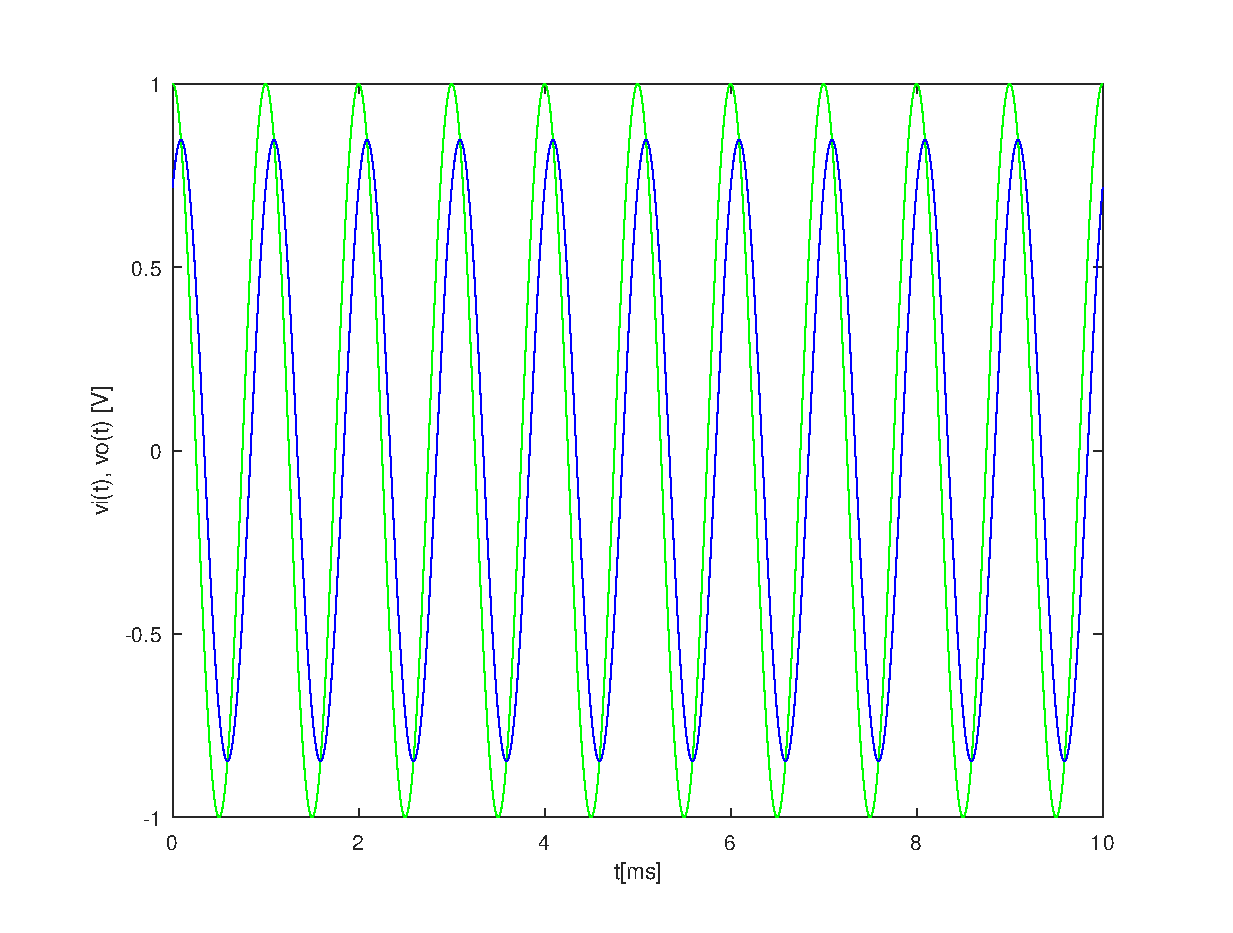
\includegraphics[width=0.8\linewidth]{forced.eps}
\caption{------------}
\label{fig:forced}
\end{figure}
